\chapter{Background on Neural Networks and Transformers}\label{ch:neural-networks}
Detailed presentation on the theoretical results of ANN will be the focus of this chapter. Starting with the discussion on different types of \textit{neurons} and a brief history about it. In Section \ref{sec:topologyann}, these neurons are then arranged to form networks which will be the topology of feedforward \textit{multilayer perceptron} (MLP). Following that, are definitions of the standard notations for ANN used for the rest of this thesis. Then what follows is the optimization on the parameters. And finally, the extension to Bayesian framework for ANN.
\section{Perceptron}
From \citeA{Haykin1998}, some 15 years after the publication of \citeA{mccullochpitts} classic paper, a new approach to the pattern recognition was introduced by (Rosenblatt 1958) in his work on the \textit{perceptron}, a novel method of supervised learning. The crowning achievement's of Rosenblatt's work was the so-called \textit{perceptron convergence theorem}, the first proof for which was outlined by (Rosenblatt 1960b).

\begin{figure}[!h]
\centering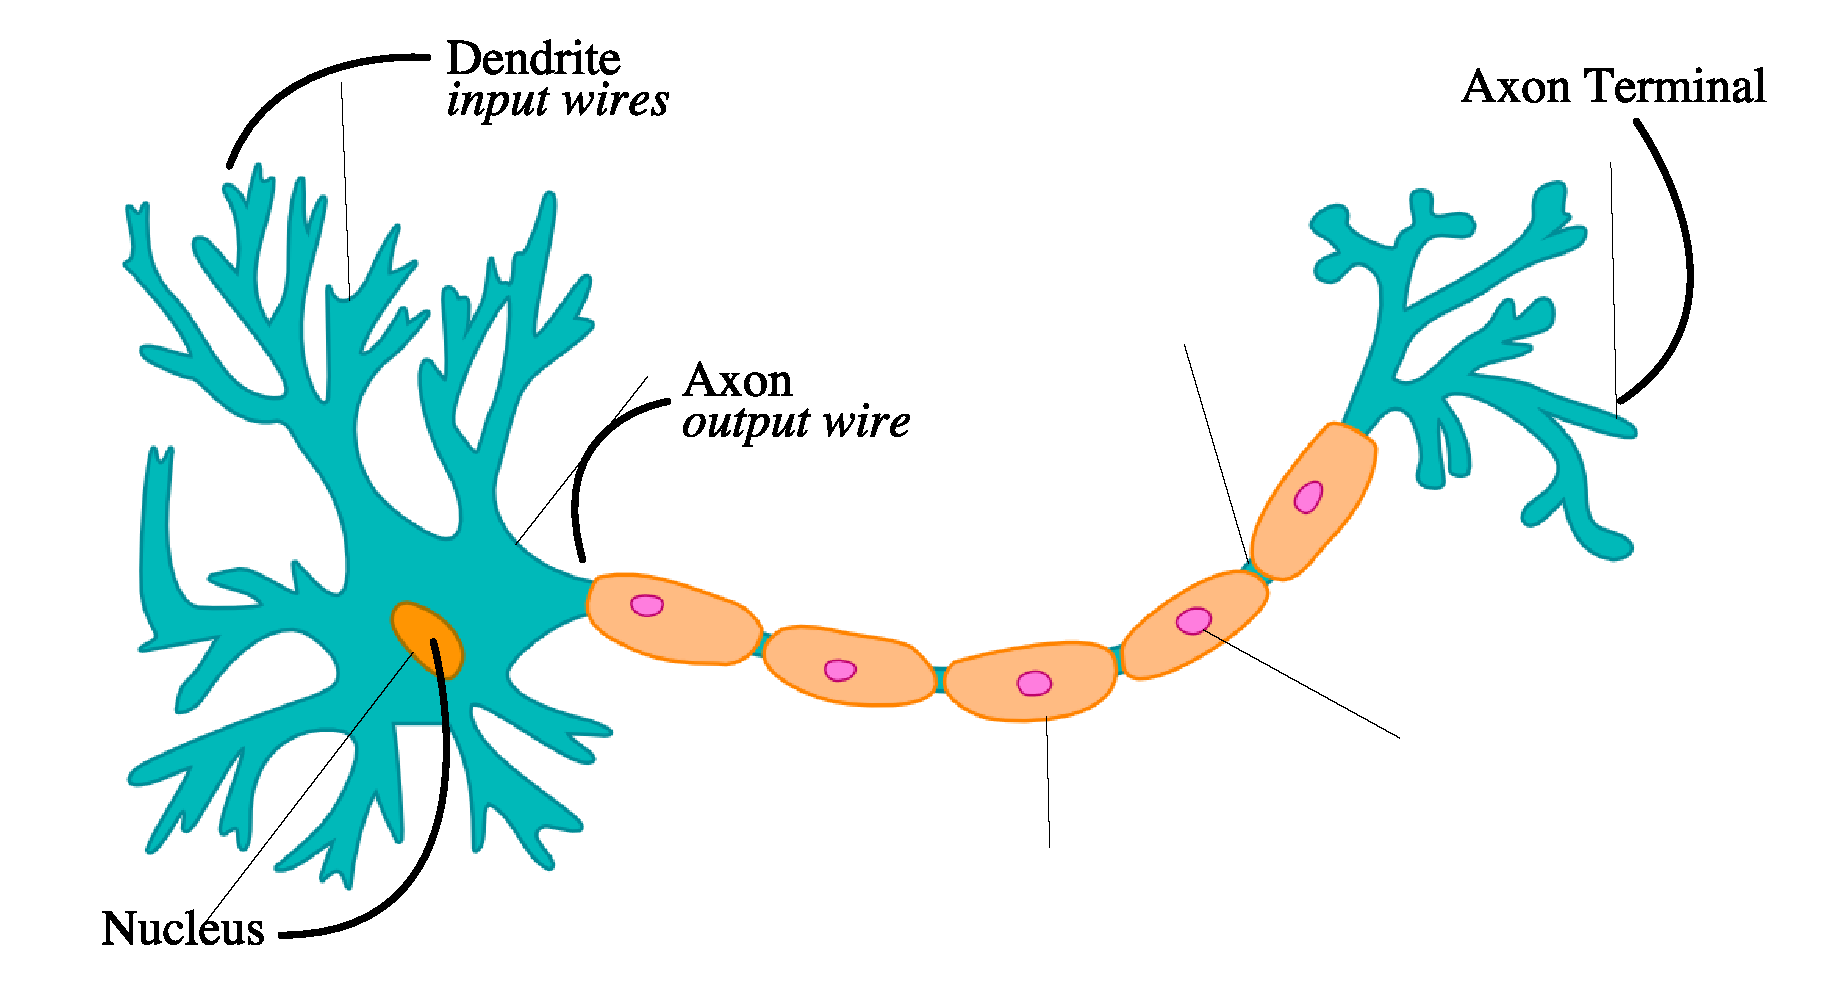
\includegraphics[scale = .4]{img/Neuron.pdf}
\caption[Structure of a Typical Biological Neuron]{Structure of a Typical Biological Neuron.\protect\footnotemark}
\label{fig:neuron}
\end{figure}

\footnotetext{Original SVG image by Quasar Jarosz but colors and some labels were modified for this paper.}

Figure \ref{fig:neuron} is the typical nerve cell in Biology. In relation to perceptron, the dendrite in this case takes several binary inputs, and returns a single binary output on its axon. Mathematically, let $w_1,w_2,\cdots,w_p$ be the parameters or weights, and $x_1,x_2,\cdots, x_p$ be the inputs. Then the perceptron is defined as follows:

\begin{equation}
\label{eq:perceptron}
\begin{aligned}
y&=
\begin{cases}
0,& \sum_{i}w_i x_i\leq c\\
1,& \sum_{i}w_i x_i> c\\
\end{cases}
\end{aligned}
\end{equation}

where $c$ is a threshold set by the experimenter. The following diagram in Figure \ref{fig:perceptron} is the schematic representation of Equation (\ref{eq:perceptron}).

\begin{figure}[!h]
\centering\begin{tikzpicture}[
init/.style={
  draw,
  circle,
  inner sep=2pt,
  font=\Huge,
  join = by -latex
},
squa/.style={
  draw,
  inner sep=2pt,
  font=\Large,
  join = by -latex
},
start chain=4,node distance=13mm,thick
]
\begin{scope}[start chain=1]
\node[on chain=1] at (0,2.5cm) 
  (x1) {$x_1$};
\node[on chain=1,join=by o-latex] 
  (w1) {$w_1$};
\end{scope}

\begin{scope}[start chain=2]
\node[on chain=2] at (0,1.5cm) 
  (x2) {$x_2$};
\node[on chain=2,join=by o-latex] 
  (w2) {$w_2$};
\end{scope}

\begin{scope}[start chain=3, node distance = 18mm]
\node[on chain=3] at (0,.7cm) 
  {$\vdots$};
\node[on chain=3] at (0,.7cm) 
  {$\vdots$};
\end{scope}

\node[on chain=4] 
  (xi) {$x_i$};
\node[on chain=4,join=by o-latex] 
  (wi) {$w_i$};
\node[on chain=4,init] (sigma) 
  {$\displaystyle\Sigma$};
\node[on chain=4,label=above:Output,join=by -latex] 
  {$y$};

\begin{scope}[start chain=5,node distance=18mm]
\node[on chain=5] at (0,-.7cm) 
  {$\vdots$};
\node[on chain=5] at (0,-.7cm) 
  {$\vdots$};
\end{scope}

\begin{scope}[start chain=6]
\node[on chain=6] at (0,-1.5cm) 
  (xp) {$x_p$};
\node[on chain=6,label=below:Parameters,join=by o-latex] 
  (wp) {$w_p$};
\end{scope}


\draw[-latex] (w1) -- (sigma);
\draw[-latex] (w2) -- (sigma);
\draw[-latex] (wi) -- (sigma);
\draw[-latex] (wp) -- (sigma);

\draw[decorate,decoration={brace,mirror}] (x1.north west) -- node[left=10pt] {Inputs} (xp.south west);
\end{tikzpicture}
\caption[Schematic Representation of the Perceptron Neuron]{Schematic Representation of the Perceptron Neuron.}
\label{fig:perceptron}
\end{figure}

One limitation of the perceptron is its binary output, which sometimes is poor in discrimination problem, such as in imaging. To address this issue, a new artificial neuron is proposed that returns continuous values between 0 and 1, and so it can be interpreted as probabilities.

\section{Logistic Sigmoid Neuron}\label{sec:sln}
The logistic sigmoid neuron or simply sigmoid neuron takes its name from the fact that it uses logistic function as its link/basis function, thus it is also known as logistic neuron. Formally, let $w_0$ be the intercept or the bias term and as before let $w_1,w_2,\cdots,w_p$ be the parameters, then the logistic sigmoid function is given by
\begin{equation}\label{eq:logsig}
z=\sum_{i}w_ix_i+w_0,\quad y=\af(z)=\frac{1}{1+\exp(-z)}
\end{equation}

In the proceeding section, the connections between neurons will be discussed, and how the architecture of these networks is designed.

\section{Topology}\label{sec:topologyann}
The basic architecture of the network comprises of the \textit{input} and the \textit{output} layers, between them are the \textit{hidden} layers. These hidden layers are layers that are not observed by the experimenter, hence the name. Figure \ref{fig:neuralnetarch} shows the diagram of a \textit{feedforward} neural network. It is feedforward due to the fact that the inputs are propagated onto the succeeding layers up to the output without redirecting back to the previous layer after processing. Otherwise the model is called \textit{recurrent} neural network. 
\begin{figure}[!h]
\tikzset{%
  every neuron/.style={
    circle,
    draw,
    minimum size=.85cm
  },
  neuron missing/.style={
    draw=none, 
    scale=4,
    text height=0.333cm,
    execute at begin node=\color{black}$\vdots$
  },
}

\centering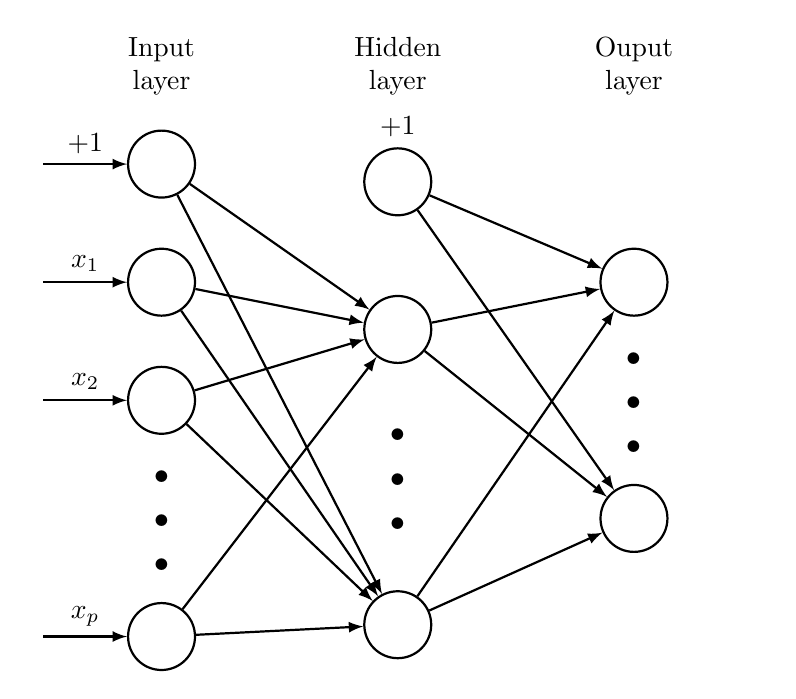
\begin{tikzpicture}[x=1.5cm, y=1.5cm, >=latex,thick]

\foreach \m/\l [count=\y] in {0,1,2,missing,3}
  \node [every neuron/.try, neuron \m/.try] (input-\m) at (0,2.5-\y) {};

\foreach \m [count=\y] in {0,1,missing,2}
  \node [every neuron/.try, neuron \m/.try ] (hidden-\m) at (2,2.6-\y*1.25) {};

\foreach \m [count=\y] in {1,missing,2}
  \node [every neuron/.try, neuron \m/.try ] (output-\m) at (4,1.5-\y) {};

\draw [<-] (input-0) -- ++(-1,0) node [above, midway] {$+1$};
\node [above] at (hidden-0.north) {$+1$};
\foreach \l [count=\i] in {1,2,p}
  \draw [<-] (input-\i) -- ++(-1,0)
    node [above, midway] {$x_{\l}$};

\foreach \i in {0,...,3}
  \foreach \j in {1,...,2}
    \draw [->] (input-\i) -- (hidden-\j);

\foreach \i in {0,...,2}
  \foreach \j in {1,...,2}
    \draw [->] (hidden-\i) -- (output-\j);

\foreach \l [count=\x from 0] in {Input, Hidden, Ouput}
  \node [align=center, above] at (\x*2,2) {\l \\ layer};

\end{tikzpicture}
\caption[Feedforward Neural Network]{Feedforward Neural Network.}
\label{fig:neuralnetarch}
\end{figure}

Since the input and output layers are at best observed, the hidden layers will only serve as behind-the-scene computations. And the parameter associated with each neuron has no interpretation at all, and that's one major limitation of ANN. Neural networks can have several hidden layers depending on the study, for high level of abstraction one might consider multiple layers also known as \textit{multilayer perceptrons} (MLP), which is a misnomer since layers are made up of logistic sigmoid neurons not of perceptrons. Networks with 2 or more hidden layers are often referred to as \textit{deep neural networks} \cite{nndeepl}, an example of this is depicted in Figure \ref{fig:deepnn}. The unknown vector $\mathbf{w}=[(w_i)]_{i=0}^p$ in Equation (\ref{eq:logsig}), is the parameter vector that needs to be estimated. And this is done by maximum likelihood which is equivalent to minimization of the error function through mathematical programming using methods such as \textit{Gradient Descent} algorithm. The succeeding section will formalize the standard notations, and then the definition of the loss function which will be the basis for choosing the best estimates of the weights, and finally the estimation.

\noindent
\begin{figure}[!h]
\tikzset{%
  every neuron/.style={
    circle,
    draw,
    minimum size=.85cm
  },
  neuron missing/.style={
    draw=none, 
    scale=4,
    text height=0.333cm,
    execute at begin node=\color{black}$\vdots$
  },
}
\centering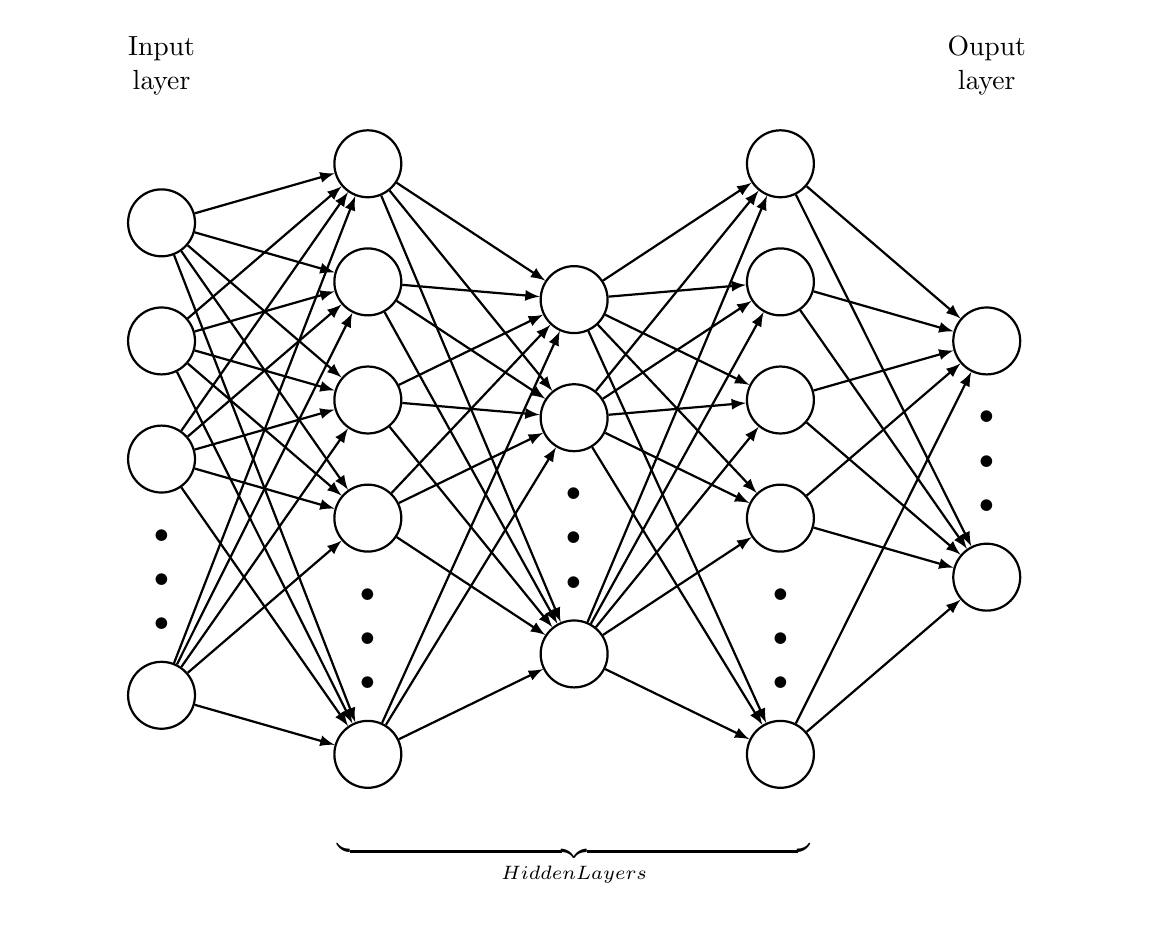
\begin{tikzpicture}[x=1.31cm, y=1.5cm, >=latex,thick]

\foreach \m/\l [count=\y] in {1,2,3,missing,4}
  \node [every neuron/.try, neuron \m/.try] (input-\m) at (0,2-\y) {};

\foreach \m [count=\y] in {1,2,3,4,missing,5}
  \node [every neuron/.try, neuron \m/.try ] (hidden1-\m) at (2,2.5-\y) {};

\foreach \m [count=\y] in {1,2,missing,3}
  \node [every neuron/.try, neuron \m/.try ] (hidden2-\m) at (4,1.35-\y) {};

\foreach \m [count=\y] in {1,2,3,4,missing,5}
  \node [every neuron/.try, neuron \m/.try ] (hidden3-\m) at (6,2.5-\y) {};

\foreach \m [count=\y] in {1,missing,2}
  \node [every neuron/.try, neuron \m/.try ] (output-\m) at (8,1-\y) {};

\foreach \i in {1,...,4}
  \foreach \j in {1,2,3,4,...,5}
    \draw [->] (input-\i) -- (hidden1-\j);

\foreach \i in {1,2,3,4,...,5}
  \foreach \j in {1,2,...,3}
    \draw [->] (hidden1-\i) -- (hidden2-\j);

\foreach \i in {1,2,...,3}
  \foreach \j in {1,2,3,4,...,5}
    \draw [->] (hidden2-\i) -- (hidden3-\j);

\foreach \i in {1,2,3,4,...,5}
  \foreach \j in {1,...,2}
    \draw [->] (hidden3-\i) -- (output-\j);

\foreach \l [count=\x from 0] in {Input, Ouput}
  \node [align=center, above] at (\x*8,2) {\l \\ layer};

\draw (4,-4.7) node[above] {$\underbrace{\hspace{6cm}}_{\text{\small Hidden Layers}}$};
\end{tikzpicture}
\caption[Multilayer Feedforward Neural Network]{Multilayer Feedforward Neural Network.}
\label{fig:deepnn}
\end{figure}

\subsection{Notations}
The following definition will serve as the standard notation for the rest of the succeeding chapters. To start with, let $f:\mathcal{X}\to\mathcal{Y}$ be the unknown \textit{target function} of the data points in the population, that is $y=f(\mathbf{x})$. The sample data set from this population is denoted by $(\mathbf{x}_1,y_1),\cdots,(\mathbf{x}_N,y_N)$. The learning algorithm picks $g:\mathcal{X}\to \mathcal{Y}$ as the \textit{final hypothesis} from the hypothesis set $\mathscr{H}=\{h_v:h_v(\mathbf{x})=\hat{y},v=1,2,\cdots,V\}$ such that $g\approx f$, that is, $g$ is the hypothesis that best approximate the target function $f$, thus $\hat{y}=g(\mathbf{x})$. The error in the training data set named ``in-sample error'' is denoted by $\ein$, while the error in the validation data set named ``out-of-sample error'' is denoted by $\eout$.

For ANN models, let $i, j$ and $l$ be the indices of the observations in the inputs, outputs and the layers containing the observations, respectively. The domain of these indices are as follows: $i\in[0,d^{(l-1)}]$, $j\in[1,d^{(l)}]$ and $l\in[1,L]$, where $d^{(l)}$ is the dimension of the outputs in the $l$th layer. The upper bound of the inputs is $d^{(l-1)}$, since this is the dimension of the outputs in the previous layer, $l-1$, and is now an input layer due to the foward-propagation process, in this case the next layer has $d^{(l)}$ dimension. Further, the lower bound of the input is 0 to account for the intercept term $w_0$. Hence the following is the standard notation of the parameters,
$$
w_{ji}^{(l)}=\begin{cases}
1\leq l \leq L&\mathrm{layers}\\
0\leq i\leq d^{(l-1)}&\mathrm{inputs}\\
1\leq j\leq d^{(l)}&\mathrm{outputs}
\end{cases}
$$

Let $\mathbf{x}_k$ be the training input, $k=1,2,\cdots,K$. Since the input layer is the $0$th layer with $d$ dimension, then each input is a $d^{(0)}\times 1$ vector. That is,
$$
\mathbf{x}_k=\left[
\begin{array}{c}
x_{ki}^{(0)}\\
x_{k2}^{(0)}\\
\vdots\\
x_{kd^{(0)}}^{(0)}
\end{array}
\right]
$$

For example in imaging, each entry in the vector corresponds to the gradient of grayscale pixel. In this setting, $h(\mathbf{x}_k,\mathbf{w})$ denotes the hypothesis or the model, where $\mathbf{w}$ is the vector of all weights. So different network achitecture relates to different model, and the final hypothesis is denoted by $g(\mathbf{x}_k,\mathbf{w})$. 

The feedforward process executes as follows: the vector $\mathbf{x}_k$ will serve as an input on the first hidden layer, whose output will then be the input on the next hidden layer, and so on until the output layer. In general,
$$
x_{kj}^{(l)}=\af\left(z_{kj}^{(l)}\right)=\af\left(\left\{\mathbf{w}_{j}^{(l)}\right\}^{\text{T}}\mathbf{x}_k^{(l-1)} + w_{j0}^{(l)}\right)=\af\left(\sum_{i=1}^{d^{(l-1)}}w_{ji}^{(l)}x_{ki}^{(l-1)}+w_{j0}^{(l)}\right),
$$
where $\mathbf{w}_{j}^{(l)}=\left[\begin{array}{cccc}w_{j1}^{(1)}&w_{j2}^{(2)}&\cdots&w_{jd^{(l-1)}}^{(l)}\end{array}\right]^{\text{T}}$. This is done recursively, that is the output $x_{kj}^{(l)}$ will be the input on the next layer. For example, the following is the formula for obtaining $x_{kj}^{(l+1)}$,
$$
\begin{aligned}
x_{kj}^{(l+1)}&=\af\left(z_{kj}^{(l+1)}\right)=\af\left(\left\{\mathbf{w}_{j}^{(l+1)}\right\}^{\text{T}}\mathbf{x}_k^{(l)} + w_{j0}^{(l)}\right)=\af\left(\sum_{i=1}^{d^{(l)}}w_{ji}^{(l+1)}x_{ki}^{(l)}+w_{j0}^{(l+1)}\right)\\
&=\af\left\{\sum_{i=1}^{d^{(l)}}w_{ji}^{(l+1)}\left[\af\left(\sum_{i=1}^{d^{(l-1)}}w_{ji}^{(l)}x_{ki}^{(l-1)}+w_{j0}^{(l)}\right)\right]+w_{j0}^{(l+1)}\right\}.
\end{aligned}
$$
So the dimension $d$ will vary from layer to layer. Consider Figure \ref{fig:neuralnetarch}, the neurons can now be labelled with the standard notations as in Figure \ref{fig:nnlab}.
So that $x_{kj}^{(1)}$ in the hidden layer has the following form:
$$
x_{kj}^{(1)}=\af(z_{kj}^{(1)})=\af\left(\left\{\mathbf{w}_{j}^{(1)}\right\}^{\text{T}}\mathbf{x}_k^{(0)} + w_{j0}^{(1)}\right)=\af\left(\sum_{i=1}^{d^{(0)}}w_{ji}^{(1)}x_{ki}^{(0)}+w_{j0}^{(1)}\right),
$$
The $x_{kj}^{(2)}$ in the output layer is computed from the following equation,
$$
\begin{aligned}
x_{kj}^{(2)}&=\af(z_{kj}^{(2)})=\af\left(\left\{\mathbf{w}_{j}^{(2)}\right\}^{\text{T}}\mathbf{x}_k^{(1)} + w_{j0}^{(2)}\right)=\af\left(\sum_{i=1}^{d^{(1)}}w_{ji}^{(2)}x_{ki}^{(1)}+w_{j0}^{(2)}\right)\\
&=\af\left\{\sum_{i=1}^{d^{(1)}}w_{ji}^{(2)}\left[\af\left(\sum_{i=1}^{d^{(0)}}w_{ji}^{(1)}x_{ki}^{(0)}+w_{j0}^{(1)}\right)\right]+w_{j0}^{(2)}\right\}.
\end{aligned}
$$

\begin{figure}[!h]
\tikzset{%
  every neuron/.style={
    circle,
    draw,
    minimum size=.85cm
  },
  neuron missing/.style={
    draw=none, 
    scale=4,
    text height=0.333cm,
    execute at begin node=\color{black}$\vdots$
  },
}

\centering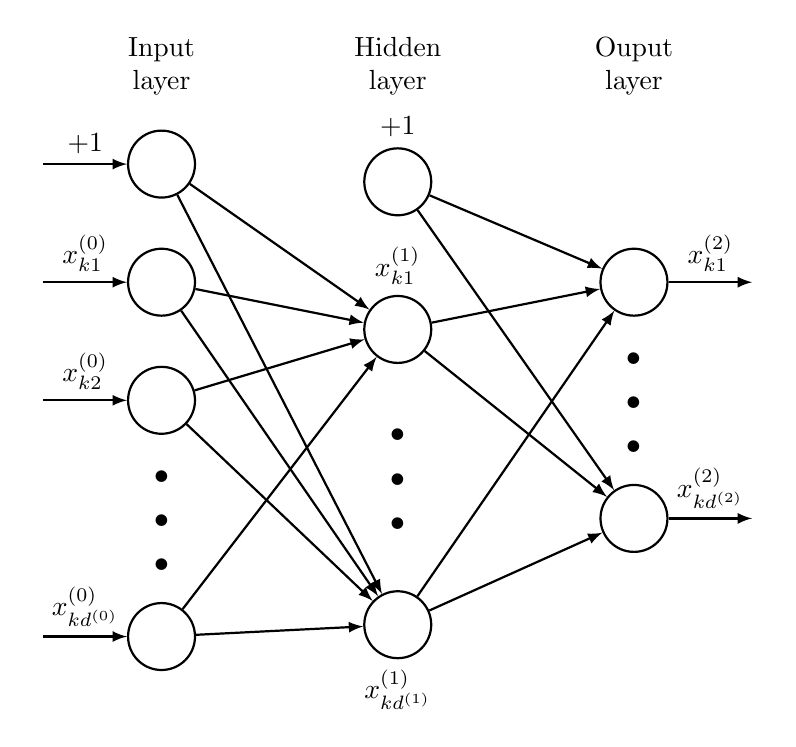
\begin{tikzpicture}[x=1.5cm, y=1.5cm, >=latex, thick]

\foreach \m/\l [count=\y] in {0,1,2,missing,3}
  \node [every neuron/.try, neuron \m/.try] (input-\m) at (0,2.5-\y) {};

\foreach \m [count=\y] in {0,1,missing,2}
  \node [every neuron/.try, neuron \m/.try ] (hidden-\m) at (2,2.6-\y*1.25) {};

\foreach \m [count=\y] in {1,missing,2}
  \node [every neuron/.try, neuron \m/.try ] (output-\m) at (4,1.5-\y) {};

  \draw [<-] (input-0) -- ++(-1,0) node [above, midway] {$+1$};
\foreach \l [count=\i] in {1,2,d^{(0)}}
  \draw [<-] (input-\i) -- ++(-1,0)
    node [above, midway] {$x_{k\l}^{(0)}$};

%\foreach \l [count=\i] in {1,missing}
  \node [above] at (hidden-0.north) {$+1$};
  \node [above] at (hidden-1.north) {$x_{k1}^{(1)}$};
  \node [below] at (hidden-2.south) {$x_{kd^{(1)}}^{(1)}$};

\foreach \l [count=\i] in {1,d^{(2)}}
  \draw [->] (output-\i) -- ++(1,0)
    node [above, midway] {$x_{k\l}^{(2)}$};

\foreach \i in {0,...,3}
  \foreach \j in {1,...,2}
    \draw [->] (input-\i) -- (hidden-\j);

\foreach \i in {0,...,2}
  \foreach \j in {1,...,2}
    \draw [->] (hidden-\i) -- (output-\j);

\foreach \l [count=\x from 0] in {Input, Hidden, Ouput}
  \node [align=center, above] at (\x*2,2) {\l \\ layer};

\end{tikzpicture}
\caption[Neural Net with Standard Neuron Notation]{Neural Net with Standard Neuron Notation.}
\label{fig:nnlab}
\end{figure}

The final output $\mathbf{x}_{k}^{(2)}$ is the value of the hypothesis, that is $h(\mathbf{x}_k,\mathbf{w})=\mathbf{x}_{k}^{(L)}$, where $L=2$.
\section{Network Training}
Network parameter estimation is done through optimization, this is because ANN loss function has no unique stationary point. That is, it consist of local minima and often one unique global minimum.
\subsection{Loss Function}\label{sec:costfun}
In this section, the error functions of ANN models for regression and classification are derived from probabilistic perspective, this will be useful when extending the model to full Bayesian treatment. For regression setup, the network has at least two nodes (one for the intercept and one for the independent variable) at the input layer and one node at the output layer. The standard activation function is the identity function, i.e. $h(\mathbf{x}_k,\mathbf{w})=z_k=\mathbf{w}^{\mathrm{T}}\mathbf{x}_k$, so there is no hidden layer, see Figure \ref{fig:slrnn}. 
\begin{figure}[t]
\centering\begin{tikzpicture}[
init/.style={
  draw,
  circle,
  inner sep=2pt,
  font=\Huge,
  join = by -latex
},
squa/.style={
  draw,
  inner sep=2pt,
  font=\Large,
  join = by -latex
},
start chain=4,node distance=13mm, thick
]
\begin{scope}[start chain=1]
\node[on chain=1] at (0,2.5cm) 
  (x1) {$x_{k1}^{(0)}$};
\node[on chain=1,join=by o-latex] 
  (w1) {$w_{11}^{(1)}$};
\end{scope}

\begin{scope}[start chain=2]
\node[on chain=2] at (0,1.5cm) 
  (x2) {$x_{k2}^{(0)}$};
\node[on chain=2,join=by o-latex] 
  (w2) {$w_{12}^{(1)}$};
\end{scope}

\begin{scope}[start chain=3, node distance = 20mm]
\node[on chain=3] at (0,.7cm) 
  {$\vdots$};
\node[on chain=3] at (0,.7cm) 
  {$\vdots$};
\end{scope}

\node[on chain=4] 
  (xi) {$x_{ki}^{(0)}$};
\node[on chain=4,join=by o-latex] 
  (wi) {$w_{1i}^{(1)}$};
\node[on chain=4,init] (sigma) 
  {$\displaystyle\Sigma$};
\node[on chain=4,label=above:Output,join=by -latex] 
  {$h(\mathbf{x},\mathbf{w})$};

\begin{scope}[start chain=5,node distance=20mm]
\node[on chain=5] at (0,-.7cm) 
  {$\vdots$};
\node[on chain=5] at (0,-.7cm) 
  {$\vdots$};
\end{scope}

\begin{scope}[start chain=6]
\node[on chain=6] at (0,-1.5cm) 
  (xp) {$x_{kd^{(0)}}^{(0)}$};
\node[on chain=6,label=below:Parameters,join=by o-latex] 
  (wp) {$w_{1d^{(0)}}^{(1)}$};
\end{scope}

\node[label=above:\parbox{2cm}{\centering Intercept \\ $w_0$}] at (sigma|-w2) (b) {};

\draw[-latex] (w1) -- (sigma);
\draw[-latex] (w2) -- (sigma);
\draw[-latex] (wi) -- (sigma);
\draw[-latex] (wp) -- (sigma);
\draw[o-latex] (b) -- (sigma);

\end{tikzpicture}
\caption[Neuron's Schematic Diagram for Linear Regression]{Neuron's Schematic Diagram for Linear Regression.}
\label{fig:slrnn}
\end{figure}
Given the training input $\mathbf{X}=[\mathbf{x}_1^{(0)},\mathbf{x}_2^{(0)},\cdots,\mathbf{x}_N^{(0)}]$, where $\mathbf{x}_k^{(0)}$ is a $d^{(0)}$-dimensional feature vector whose elements are $x_{k0}^{(0)},x_{k1}^{(0)},\cdots, x_{kd^{(0)}}^{(0)}\;\forall k=1,2,\cdots,K$, the corresponding target variable is $\mathbf{Y}=[y_1,y_2,\cdots,y_N]^{\mathrm{T}}$, and the error term $\varepsilon_k$ is assumed to be normally distributed with mean $\ev\varepsilon_k=0$ and variance $\var\varepsilon_k=\sigma^2$. It follows that the uncertainty around the target variable is also Gaussian distributed and is given by
\begin{align}
p(y|\mathbf{x},\mathbf{w},\sigma^2)&=\mathcal{N}(y|h(\mathbf{x},\mathbf{w}),\sigma^2)\nonumber\\
&=\frac{1}{\sqrt{2\pi\sigma^{2}}}\exp\left[-\frac{(y-h(\mathbf{x},\mathbf{w}))^2}{2\sigma^{2}}\right]
\end{align}
If the data are independent and identically distributed, then the likelihood function of $\mathbf{y}$ is given by,
\begin{align}
\mathcal{L}(\mathbf{w},\sigma|\mathbf{y},\mathbf{X})&=p(\mathbf{y}|\mathbf{X},\mathbf{w},\sigma)=\prod_{k=1}^{K}\mathcal{N}(y_k|h(\mathbf{x}_k,\mathbf{w}),\sigma^2)\nonumber\\
&=\frac{1}{(2\pi)^{K/2}\sigma^K}\exp\left[-\frac{1}{2\sigma^2}\sum_{k=1}^{K}(y_k-h(\mathbf{x}_k,\mathbf{w}))^2\right].
\end{align}
Taking the log-likelihood,
\begin{equation}
\label{eq:mle}
\ell(\mathbf{w},\sigma|\mathbf{y},\mathbf{X})=-\frac{1}{2\sigma^2}\sum_{k=1}^K(y_k-h(\mathbf{x}_k,\mathbf{w}))^2-K\log\sigma-\frac{K}{2}\log 2\pi.
\end{equation}
The estimate for the weight $\mathbf{w}$, denoted by $\hat{\mathbf{w}}_{\mathrm{MLE}}$, is obtained by maximizing the log-likelihood function. To do so, partial differentiation is applied to Equation (\ref{eq:mle}) with respect to $\mathbf{w}$, suggesting that the last two terms in the right hand side can be disregarded since these are not dependent on $\mathbf{w}$. Also, the location of the maximum log-likelihood with respect to $\mathbf{w}$ is not affected by arbitrary positive scalar multiplication, so the factor $\frac{1}{\sigma^2}$ can be omitted. Equivalently, one can minimize the negative log-likelihood instead of maximizing $\ell$. The reason for doing this has something to do with numerical computation, since optimizers in most statistical packages often work by minimizing the function. Thus differentiating negative of Equation (\ref{eq:mle}) is the same as differentiating the following equation,
\begin{equation}
\label{eq:regin}
\ein(h)=\frac{1}{2}\sum_{k=1}^K(y_k-h(\mathbf{x}_k,\mathbf{w}))^2,
\end{equation}
which is similar to the form of \textit{residual sum-of-squares}. Hence the sum-of-squares error function is a consequence of maximum likelihood under the normality assumption of the uncertainty around the target variable.

Likewise, the precision parameter can be estimated using maximum likelihood, by simply differentiating Equation (\ref{eq:mle}) with respect to $\sigma$, i.e.
$$
\hat{\sigma}_{\mathrm{mle}}^2=\frac{1}{K}\sum_{k=1}^K(y_k-h(\mathbf{x}_k,\mathbf{w}))^2.
$$

Now consider the case for classification, in which there is a single target variable $y$ that returns binary output, cases like when $y=1$ corresponds to class $\mathcal{C}_1$ and $y=0$ for class $\mathcal{C}_2$. The appropriate activation function is the logistic sigmoid defined in Section \ref{sec:sln} that is 
$$
\af(z)=\frac{1}{1+\exp(-z_k)},
$$
implying $\af:\mathbb{R}\to[0,1]$, and hence it can be interpreted as probability, this type of model has the same network architecture and neuron's schematic diagram as that in linear regression model (see Figure \ref{fig:slrnn}), but this time the activation function has unit interval range with hypothesis given by
$$\hat{y}=h(\mathbf{x},\mathbf{w})=\begin{cases}
1,&\af>c\\
0,&\af\leq c
\end{cases},$$
where $c$ is specified by the user, and is often chosen to be 0.5. 

\begin{figure}[t]
\centering\begin{tikzpicture}[
init/.style={
  draw,
  circle,
  inner sep=2pt,
  font=\Huge,
  join = by -latex
},
squa/.style={
  draw,
  inner sep=2pt,
  font=\Large,
  join = by -latex
},
squa1/.style={
  draw,
  inner sep=2pt,
  join = by -latex
},
start chain=4,node distance=13mm, thick
]
\begin{scope}[start chain=1]
\node[on chain=1] at (0,2.5cm) 
  (x1) {$x_{k1}^{(0)}$};
\node[on chain=1,join=by o-latex] 
  (w1) {$w_{11}^{(1)}$};
\end{scope}

\begin{scope}[start chain=2]
\node[on chain=2] at (0,1.5cm) 
  (x2) {$x_{k2}^{(0)}$};
\node[on chain=2,join=by o-latex] 
  (w2) {$w_{12}^{(1)}$};

\end{scope}

\begin{scope}[start chain=3, node distance = 20mm]
\node[on chain=3] at (0,.7cm) 
  {$\vdots$};
\node[on chain=3] at (0,.7cm) 
  {$\vdots$};
\end{scope}

\node[on chain=4] 
  (xi) {$x_{ki}^{(0)}$};
\node[on chain=4,join=by o-latex] 
  (wi) {$w_{1i}^{(1)}$};
\node[on chain=4,init] (sigma) 
  {$\displaystyle\Sigma$};
\node[on chain=4,squa,label=above:{\parbox{2cm}{\centering Activation \\ function}}]   
  (af) {$\af$};
\node[on chain=4,squa1]
  (con) {if $\af>c$};

\begin{scope}[start chain=5,node distance=20mm]
\node[on chain=5] at (0,-.7cm) 
  {$\vdots$};
\node[on chain=5] at (0,-.7cm) 
  {$\vdots$};
\end{scope}

\begin{scope}[start chain=6]
\node[on chain=6] at (0,-1.5cm) 
  (xp) {$x_{kd^{(0)}}^{(0)}$};
\node[on chain=6,label=below:Parameters,join=by o-latex] 
  (wp) {$w_{1d^{(0)}}^{(1)}$};
\end{scope}

\node[label=above:\parbox{2cm}{\centering Intercept \\ $w_0$}] at (sigma|-w1) (b) {};
\node at (9.5,1.6cm) {True};
\node at (11.5,1.3cm) (tr) {$\hat{y}=1$};
\node at (11.5,-1.3cm) (fl) {$\hat{y}=0$};
\node at (9.5,-1.6cm) {False};
\draw[-latex] (w1) -- (sigma);
\draw[-latex] (w2) -- (sigma);
\draw[-latex] (wi) -- (sigma);
\draw[-latex] (wp) -- (sigma);
\draw[o-latex] (b) -- (sigma);
\draw[-latex] (con) |- (tr);
\draw[-latex] (con) |- (fl);

\end{tikzpicture}
\caption[Neuron's Schematic Diagram for Logistic Regression]{Neuron's Schematic Diagram for Logistic Regression.}
\label{fig:logrnn}
\end{figure}

The probability of success, in this case $y=1$ for $\mathcal{C}_1$ is 
$$
p(y=1|h(\mathbf{x},\mathbf{w}))=h(\mathbf{x},\mathbf{w})
$$
So that the conditional distribution of the target variable $y$ given $\mathbf{x}$ is a Bernoulli distribution with density given by
$$
p(y|h(\mathbf{x},\mathbf{w}))=\mathcal{B}(y|h(\mathbf{x},\mathbf{w}))=h(\mathbf{x},\mathbf{w})^{y}(1-h(\mathbf{x},\mathbf{w}))^{1-y},\quad y\in\{0,1\}.
$$

So for sample data set $\{\mathbf{x}_k,y_k\}$ where $\mathbf{x}_k$ is a $d^{(0)}$-dimensional feature space and $y_k\in\{0,1\}\;\forall k=1,\cdots, K$, if the $y$s are independent and identically distributed then the likelihood function is given by
$$
\mathcal{L}(h(\mathbf{x}_k,\mathbf{w})|\mathbf{y})=\prod_{k=1}^{K}h(\mathbf{x}_k,\mathbf{w})^{y_k}(1-h(\mathbf{x}_k,\mathbf{w}))^{1-y_k},
$$
and the negative log-likelihood is given by 
\begin{align}
\ein(h)&=-\ell (h(\mathbf{x}_k,\mathbf{w})|\mathbf{y})\nonumber\\
&=-\sum_{k=1}^{K}\left[y_k\log h(\mathbf{x}_k,\mathbf{w})+(1-y_k)\log(1-h(\mathbf{x}_k,\mathbf{w}))\right].\label{eq:logitein}
\end{align}
This equation is known as \textit{cross-entropy} loss function. 
\begin{figure}[!t]
\centering
\tikzset{%
  every neuron/.style={
    circle,
    draw,
    minimum size=.85cm
  },
  neuron missing/.style={
    draw=none, 
    scale=4,
    text height=0.333cm,
    execute at begin node=\color{black}$\vdots$
  },
}
\centering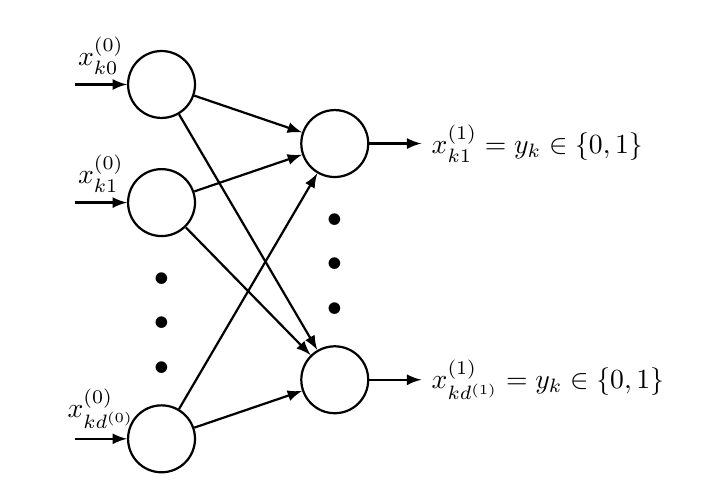
\begin{tikzpicture}[x=1.1cm, y=1.5cm, >=latex, thick]

\foreach \m/\l [count=\y] in {1,2,missing,3}
  \node [every neuron/.try, neuron \m/.try] (input-\m) at (0,1-\y) {};

\foreach \m [count=\y] in {1,missing,2}
  \node [every neuron/.try, neuron \m/.try ] (output-\m) at (2,.5-\y) {};

\foreach \l [count=\i+1] in {0,1,d^{(0)}}
  \draw [<-] (input-\i) -- ++(-1,0)
    node [above, midway] {$x_{k\l}^{(0)}$};

\foreach \l [count=\i] in {1,d^{(1)}}
  \draw [->] (output-\i) -- ++(1,0)
    node [above, right] {$x_{k\l}^{(1)}=y_k\in\{0,1\}$};

\foreach \i in {1,2,...,3}
  \foreach \j in {1,...,2}
    \draw [->] (input-\i) -- (output-\j);
\end{tikzpicture}
\caption[Neural Network for $d^{(1)}\geq 2$ Output Nodes]{Neural Network for $d^{(1)}\geq 2$ Output Nodes}
\label{fig:kloginn}
\end{figure}
Extending the case to at least two separate binary classification requires $d^{(L)}\geq 2$ neurons on the output layer, each of which has a logistic sigmoid activation function. So the target variable is defined as $\mathbf{y}_k=[y_1,y_2,\cdots,y_{d^{(L)}}]^{\mathrm{T}}$, where $y_j\in\{0,1\}\;\forall j=1,2,\cdots, d^{(L)}$. Assuming independence on the class labels, the joint conditional distribution of the targets given the input vector is
$$
p(\mathbf{y}|\mathbf{x},\mathbf{w})=\prod_{j=1}^{d^{(L)}}h(\mathbf{x},\mathbf{w})^{y_j}\left[1-h(\mathbf{x},\mathbf{w})\right]^{1-y_j}.
$$
Then the likelihood function is given by
$$
\mathcal{L}(h(\mathbf{x}_k,\mathbf{w})|\mathbf{y})=\prod_{k=1}^{K}\prod_{j=1}^{d^{(L)}}h(\mathbf{x}_{k},\mathbf{w})^{y_{kj}}\left[1-h(\mathbf{x}_{k},\mathbf{w})\right]^{1-y_{kj}}.
$$
The negative log-likelihood then becomes,
\begin{align}
\ein(h)&=-\ell (h(\mathbf{x}_{k},\mathbf{w})|\mathbf{y})\nonumber\\
&=-\sum_{k=1}^{K}\sum_{j=1}^{d^{(L)}}\left[y_{kj}\log h(\mathbf{x}_{k},\mathbf{w})+(1-y_{kj})\log(1-h(\mathbf{x}_{k},\mathbf{w}))\right].\label{eq:mlogitein}
\end{align}

In general, the loss function of a neural network can be written as the average errors of the errors in the output layer across all $k$ training inputs, i.e.
\begin{align}
\ein(h)&=\frac{1}{K}\sum_{k=1}^K\frac{1}{2}\sum_{j=1}^{d^{(L)}}(y_{kj}-h(\mathbf{x}_{k},\mathbf{w}))^2\\
&=\frac{1}{K}\sum_{k=1}^K\varepsilon(h(\mathbf{x}_{k},\mathbf{w}),y_{kj})
\end{align}

This equation is also known as the \textit{mean squared error}. In order to minimize this function, one has to consider numerical methods such as \textit{gradient descent} and \textit{stochastic gradient descent}.
\subsection{Back-propagation Algorithm}\label{sec:backprop}
The average error of the $k$ training inputs defined in Section \ref{sec:costfun} is given by
\begin{equation}\label{eq:errornn}
\ein(\mathbf{w})\triangleq\frac{1}{K}\sum_{k=1}^{K}\varepsilon(\mathbf{h}(\mathbf{x}_k,\mathbf{w}),\mathbf{y}_k).
\end{equation}
The terms in this equation are errors of the training inputs. That is, for each training input there is a corresponding error that needs to be minimized. This error is the difference between the target $\mathbf{y}_k$ and the output of the hypothesis $\mathbf{h}(\mathbf{x}_k,\mathbf{w})$. To account for the iteration counter $r$, let $\hat{\mathbf{w}}_r$ be the notation for the estimate of $\mathbf{w}$ at the $r$th iteration; also let $\varepsilon_r$ be the error at the . The inner term of Equation (\ref{eq:errornn}) can be expanded as follows:
\begin{align}
\varepsilon(\mathbf{h}(\mathbf{x}_k,\hat{\mathbf{w}}_r),\mathbf{y}_k)&\triangleq\frac{1}{2}\lVert\mathbf{y}_k-\mathbf{h}(\mathbf{x}_k,\hat{\mathbf{w}}_r)\rVert^2=\frac{1}{2}\sum_{j=1}^{d^{(L)}}(y_{kj}-h_j(\mathbf{x}_k,\mathbf{w}))^2\nonumber\\
&=\frac{1}{2}\sum_{j=1}^{d^{(L)}}\left(y_{kj}-x_{kj}^{(L)}\right)^2=\frac{1}{2}\sum_{j=1}^{d^{(L)}}\left[y_{kj}-\af\left(z_{kj}^{(L)}\right)\right]^2\nonumber\\
&=\frac{1}{2}\sum_{j=1}^{d^{(L)}}\left[y_{kj}-\af\left(\sum_{i=1}^{d^{(L-1)}}w_{ji}^{(L)}x_{ki}^{(L-1)}+w_{j0}^{(L)}\right)\right]^2.
\end{align}
For each training input $k$, gradient descent algorithm is applied to the function $\varepsilon(\mathbf{h}(\mathbf{x}_k,\mathbf{w}),\mathbf{y}_{k})$. The average of all this function correspond to the loss function, so the minimum average of the error terms will give the corresponding estimate of the parameters. For simplicity, assuming there is only one hidden layer, that is $L=2$. Consider the following:

\begin{equation}
\frac{\partial \ein(\mathbf{w})}{\partial w_{ji}^{(L)}}=\frac{\partial \ein(\mathbf{w})}{\partial \varepsilon(\mathbf{h}(\mathbf{x}_k,\mathbf{w}),\mathbf{y}_{k})}\frac{\partial \varepsilon(\mathbf{h}(\mathbf{x}_k,\mathbf{w}),\mathbf{y}_{k})}{\partial w_{ji}^{(L)}}
\end{equation}
where,
\begin{align}
\frac{\partial \ein(\mathbf{w})}{\partial \varepsilon(\mathbf{h}(\mathbf{x}_k,\mathbf{w}),\mathbf{y}_{k})}&=\frac{\partial}{\partial \varepsilon(\mathbf{h}(\mathbf{x}_k,\mathbf{w}),\mathbf{y}_{k})}\frac{1}{K}\sum_{k=1}^{K}\varepsilon(\mathbf{h}(\mathbf{x}_k,\mathbf{w}),\mathbf{y}_k)\nonumber\\
&=\frac{1}{K}\sum_{k=1}^{K}\frac{\partial}{\partial \varepsilon(\mathbf{h}(\mathbf{x}_k,\mathbf{w}),\mathbf{y}_{k})}\frac{1}{2}\sum_{j=1}^{d^{(L)}}(y_{kj}-h_j(\mathbf{x}_k,\mathbf{w}))^2\nonumber\\
&=\frac{1}{K}\sum_{k=1}^{K}\frac{\partial}{\partial \varepsilon(\mathbf{h}(\mathbf{x}_k,\mathbf{w}),\mathbf{y}_{k})}\frac{1}{2}\sum_{j=1}^{d^{(L)}}\left[y_{kj}-x_{kj}^{(L)}\right]^2\nonumber\\
&=\frac{1}{K}\sum_{k=1}^{K}\sum_{j=1}^{d^{(L)}}\left[y_{kj}-x_{kj}^{(L)}\right],\label{eq:err}
\end{align}
and
\begin{align}
\frac{\partial \varepsilon(\mathbf{h}(\mathbf{x}_k,\mathbf{w}),\mathbf{y}_{k})}{\partial w_{ji}^{(L)}}&=\frac{\partial}{\partial w_{ji}^{(L)}}\frac{1}{K}\sum_{k=1}^{K}\sum_{j=1}^{d^{(L)}}\left[y_{kj}-x_{kj}^{(L)}\right]\nonumber\\
&=\frac{1}{K}\sum_{k=1}^{K}\left[-\left(y_{kj}-x_{kj}^{(L)}\right)\frac{\partial x_{kj}^{(L)}}{\partial w_{ji}^{(L)}}\right].\label{eq:inerr}
\end{align}
And note that $x_{kj}^{(L)}=\af\!\left(z_{kj}^{(L)}\right)=\af\!\left(\sum_{i=1}^{d^{(L-1)}}w_{ji}^{(L)}x_{ki}^{(L-1)}+w_{j0}^{(L)}\right)$. Hence,
\begin{align}
\frac{\partial \ein(\mathbf{w})}{\partial w_{ji}^{(L)}}&=-\frac{1}{K}\sum_{k=1}^{K}\left(y_{kj}-x_{kj}^{(L)}\right)\frac{\partial x_{kj}^{(L)}}{\partial z_{kj}^{(L)}}\frac{\partial z_{kj}^{(L)}}{\partial w_{ji}^{(L)}}\nonumber\\
&=-\frac{1}{K}\sum_{k=1}^{K}\left(y_{kj}-x_{kj}^{(L)}\right)\af'\!\left(z_{kj}^{(L)}\right)x_{ki}^{(L-1)}.\label{eq:grad1}
\end{align}
A gradient descent update at the $(r+1)$st iteration has the form,
\begin{equation}
w_{ji,r+1}^{(L)}=w_{ji,r}^{(L)}+\Delta w_{ji,r}^{(L)}=w_{ji,r}^{(L)}-\gamma\frac{\partial \ein(h)}{\partial w_{ji,r}^{(L)}}.
\end{equation}
The $\Delta w_{ji,r}^{(L)}$ can be expressed as follows:
\begin{equation}
\Delta w_{ji,r}^{(L)}=-\gamma\frac{\partial \ein(h)}{\partial w_{ji,r}^{(L)}}=\gamma\delta_{j}^{(L)}x_{ki}^{(L-1)},
\end{equation}
where $\delta_{j}^{(L)}$ is the \textit{local gradient} defined as
\begin{align}
\delta_{j}^{(L)}&=-\frac{\partial \ein(h)}{\partial z_{kj}^{(L)}}=-\frac{\partial \ein(h)}{\partial x_{kj}^{(L)}}\frac{\partial x_{kj}^{(L)}}{\partial z_{kj}^{(L)}}=\frac{1}{K}\sum_{k=1}^{K}\varepsilon(h_j(\mathbf{x}_k,\mathbf{w}),y_{kj})\af'\!\left(z_{kj}^{(L)}\right)\nonumber\\
&=\frac{1}{K}\sum_{k=1}^{K}\left(y_{kj}-x_{kj}^{(L)}\right)\af'\!\left(z_{kj}^{(L)}\right).
\end{align}
Thus the local gradient is the product of the error signal at the $j$th neuron of the $L$th layer and the derivative of the associated activation function.

For weights at $(L-1)$th layer, the local gradient is then given by
\begin{equation}\label{eq:delta2}
\delta_{j}^{(L-1)}=-\frac{\partial \ein(h)}{\partial x_{kj}^{(L-1)}}\frac{\partial x_{kj}^{(L-1)}}{\partial z_{kj}^{(L-1)}}=-\frac{\partial \ein(h)}{\partial x_{kj}^{(L-1)}}\af'\!\left(z_{kj}^{(L-1)}\right).
\end{equation}
where,
\begin{equation}
\frac{\partial \ein(\mathbf{w})}{\partial x_{kj}^{(L-1)}}=\frac{\partial \ein(\mathbf{w})}{\partial \varepsilon(\mathbf{h}(\mathbf{x}_k,\mathbf{w}),\mathbf{y}_{k})}\frac{\partial \varepsilon(\mathbf{h}(\mathbf{x}_k,\mathbf{w}),\mathbf{y}_{k})}{\partial x_{kj}^{(L)}}\frac{\partial x_{kj}^{(L)}}{\partial z_{kj}^{(L)}}\frac{\partial z_{kj}^{(L)}}{\partial x_{kj}^{(L-1)}}.
\end{equation}
And since
\begin{equation}
\frac{\partial \ein(\mathbf{w})}{\partial \varepsilon(\mathbf{h}(\mathbf{x}_k,\mathbf{w}),\mathbf{y}_{k})}\frac{\partial \varepsilon(\mathbf{h}(\mathbf{x}_k,\mathbf{w}),\mathbf{y}_{k})}{\partial x_{kj}^{(L)}}=-\frac{1}{K}\sum_{k=1}^{K}\sum_{j=1}^{d^{(L)}}\left(y_{kj}-x_{kj}^{(L)}\right)
\end{equation}
then
\begin{align}
\frac{\partial \ein(\mathbf{w})}{\partial x_{kj}^{(L-1)}}&=-\frac{1}{K}\sum_{k=1}^{K}\sum_{j=1}^{d^{(L)}}\left(y_{kj}-x_{kj}^{(L)}\right)\frac{\partial x_{kj}^{(L)}}{\partial z_{kj}^{(L)}}\frac{\partial z_{kj}^{(L)}}{\partial x_{kj}^{(L-1)}}\nonumber\\
&=-\sum_{j=1}^{d^{(L)}}\frac{1}{K}\sum_{k=1}^{K}\left(y_{kj}-x_{kj}^{(L)}\right)\af'\!\left(z_{kj}^{(L)}\right)w_{ji}^{(L)}\nonumber\\
&=-\sum_{j=1}^{d^{(L)}}\delta_j^{(L)}w_{ji}^{(L)}.\label{eq:deltawij}
\end{align}
So that using Equation (\ref{eq:deltawij}) in (\ref{eq:delta2}),
\begin{equation}\label{eq:backprop}
\delta_{j}^{(L-1)}=\af'\!\left(z_{kj}^{(L-1)}\right)\sum_{j=1}^{d^{(L)}}\delta_j^{(L)}w_{ji}^{(L)}.
\end{equation}
And just to emphasize $\af'\!\left(z_{kj}^{(L-1)}\right)$ is indexed at $j$ but at the $(L-1)$th layer, so the dimension on that layer is not necessarily the same with the $L$th layer, and thus it is not included in the summation. Equations (\ref{eq:backprop}) is known as the \textit{back-propagation equations}.

\section{Transformers}\label{sec:transformers}
Transformer models is a model based on the work of \cite{vaswani2017attention}. These models are a type of neural network architecture designed to handle sequential data, primarily used in natural language processing (NLP) tasks. Unlike traditional recurrent neural networks (RNNs) and long short-term memory networks (LSTMs), transformers do not rely on sequential data processing. Instead, they utilize an attention mechanism that allows them to process entire sequences simultaneously, significantly improving efficiency and effectiveness.

\subsection{Attention Mechanism}
The core innovation of transformers is the self-attention mechanism, which computes attention scores to weigh the importance of different words in a sentence relative to each other. 

\begin{defn}[Vector Self-Attention]\label{defn:vec-self-attention}
    Let $\mathbf{X}:=[\mathbf{x}_1,\cdots,\mathbf{x}_N]^{\text{T}}$ be the data matrix, such that $\mathbf{x}_i\in\mathbb{R}^{D}$ is a word embedding, then the \textit{self-attention} is given by
    \begin{equation}\label{eq:self-attention}
        \mathbf{y}_n := \sum_{n=1}^{N}a_{nm}\mathbf{x}_n,
    \end{equation}
    where $0\leq a_{nm}\leq 1$ is a attention coefficient, and that $\sum_{\forall l}a_{nm}=1$.
\end{defn}

The attention weights are based on the idea of \textit{query}, \textit{key}, and \textit{value}, where given the an input vector $\mathbf{x}_n$, its similarity to other words $\mathbf{x}_n,n\neq m$. Here $\mathbf{x}_n$ is the query and $\mathbf{x}_m$ is the key. The similarity can be computed using \textit{cosine similarity} (\textit{see} discussions on this in Section \ref{sec:cosine_similarity} and Defn. \ref{defn:cosine_similarity})
\begin{defn}[Attention Coefficient]
    Let $\mathbf{X}:=[\mathbf{x}_1,\cdots,\mathbf{x}_N]^{\text{T}}$ be the data matrix, then the \textit{attention coefficient} is
    \begin{equation}
        a_{nm}:=\frac{\exp(\mathbf{x}_n^{\text{T}}\mathbf{x}_l)}{\displaystyle\sum_{m'=1}^{M}\exp(\mathbf{x}_n^{\text{T}}\mathbf{x}_{m'})},
    \end{equation}
    the softmax formula helps $a_{kl}$ satisfy its contraints.
\end{defn}
\begin{defn}[Identity Self-Attention]
    Let $\mathbf{y_1},\cdots,\mathbf{y}_N$ be the \textit{vector self-attention}, then $\mathbf{Y}=[\mathbf{y}_1,\cdots,\mathbf{y}_N]^{\text{T}}$ is the \textit{identity self-attention} with the following formula:
    \begin{equation}\label{eq:identity-self-attention}
        \mathbf{Y}:=\operatorname{Softmax}(\mathbf{X}\mathbf{X}^{\text{T}})\mathbf{X}
    \end{equation}
\end{defn}
\begin{remark}
    It is called \text{identity self-attention} since there is no learnable parameter that controls the data matrix input.
\end{remark}
\begin{defn}[Encoded Data Matrix]\label{defn:encoded-data-matrix}
    Let $\mathbf{V}\in\mathbb{R}^{D\times D}$, then the \textit{encoded data matrix} is given by $\mathbf{Z}:=\mathbf{X}\mathbf{V}$
\end{defn}
So that from Defn. \ref{defn:encoded-data-matrix}, Eq. \ref{eq:identity-self-attention} becomes:
\begin{align}
    \mathbf{Y}=&\operatorname{Softmax}(\mathbf{X}\mathbf{V}\mathbf{V}^{\text{T}}\mathbf{X}^{\text{T}})\mathbf{X}\mathbf{V}\\
    =&\operatorname{Softmax}(\mathbf{Z}\mathbf{Z}^{\text{T}})\mathbf{Z}
\end{align}
Further, it would be better to add learnable weights for the \textit{query}, \textit{key}, and \textit{value} as well. This is formulated in the next definition.
\begin{defn}[Self-Attention]\label{defn:self-attention}
    Let $\mathbf{W}_{(q)},\mathbf{W}_{(k)}$, and $\mathbf{W}_{(v)}$ be the weights matrix for \textit{query}, \textit{key}, and \textit{value}, respectively, such that $\mathbf{W_{(i)}}\in\mathbb{R}^{D\times D_i},i\in\{q,k,v\}$, then the \textit{self-attention} is 
    \begin{align}
        \mathbf{Y}=&\operatorname{Softmax}(\mathbf{Z}\mathbf{W}_{(q)}\mathbf{W}_{(k)}^{\mathbf{T}}\mathbf{Z}^{\mathbf{T}})\mathbf{Z}\mathbf{W}_{(v)}\\
        &\operatorname{Softmax}(\mathbf{Q}\mathbf{K}^{\text{T}})\mathbf{V},
    \end{align}
    where $\mathbf{Q}:=\mathbf{Z}\mathbf{W}_{(q)},\mathbf{K}:=\mathbf{Z}\mathbf{W}_{(k)},\mathbf{V}:=\mathbf{Z}\mathbf{W}_{(v)}$. The above equation will only work if $\mathbf{W}_{(q)}$ and $\mathbf{W}_{(k)}$ have the same dimention.
\end{defn}

Further, becaus the Softmax can suffer from having exponentially small gradients for inputs of high magnitude, the same case for tanh or logistic-sigmoid activation functions, scaling can be used to address this issue.

\begin{defn}[Scaled Self-Attention]
    From Defn. \ref{defn:self-attention}, the \textit{scaled self-attention} is
    \begin{equation}
        \mathbf{Y}=\operatorname{Attention}(\mathbf{Q},\mathbf{K},\mathbf{V}):=\operatorname{Softmax}\left[\frac{\mathbf{Q}\mathbf{K}^{\text{T}}}{\sqrt{D}}\right]\mathbf{V},
    \end{equation}
    where $D$ can be $D_q$ or $D_k$ since $D_q=D_k$.
\end{defn}

\subsection{Multi-Head Attention}
To enhance the model's ability to focus on different parts of the input sequence, transformers employ multi-head attention. This involves splitting the query, key, and value matrices into multiple heads, applying the attention mechanism to each head independently, and then concatenating the results.
\begin{defn}[Multi-Head Attention]
    Let $\mathbf{Y}_1,\cdots,\mathbf{Y}_H$ be the scaled self-attention such that $\mathbf{Y}_h=\operatorname{Attention}(\mathbf{Q}_h,\mathbf{K}_h,\mathbf{V}_h)$, where $\mathbf{Q}_h=\mathbf{X}\mathbf{W}_h^{(q)},\mathbf{K}_h=\mathbf{X}\mathbf{W}_h^{(k)}$, and $\mathbf{V}_h=\mathbf{X}\mathbf{V}_h^{(k)}$, then the \textit{multi-head attention} is
    \begin{equation}
        \operatorname{MultiHead}(\mathbf{Q},\mathbf{K},\mathbf{V}):=\operatorname{Concat}(\mathbf{Y}_1,\cdots,\mathbf{Y}_H)\mathbf{W}^{(o)},
    \end{equation}
    where $\operatorname{Concat}$ simply combines the outputs $\mathbf{Y}_h$ into a matrix, so that, $\mathbf{W}^{(o)}\in\mathbb{R}^{H\times D_o}$.
\end{defn}
\subsection{Positional Encoding}
Since transformers do not process input sequences in order, it require a way to incorporate the position of each word. This is achieved through positional encoding, which adds positional information to the input embeddings. Positional encodings are vectors added to the input embeddings and can be computed using sine and cosine functions of different frequencies.
\begin{defn}[Positional Encoding]
    Let $\mathbf{r}_n$ be the vector of positional encoding with components defined as:
    \begin{equation}
        r_{ni}:=\begin{cases}
            \sin\left(\displaystyle\frac{n}{L^{i/D}}\right)&\text{if}\;i\;\text{is even,}\\
            \cos\left(\displaystyle\frac{n}{L^{(i-1)/D}}\right)&\text{if}\;i\;\text{is odd},
        \end{cases}
    \end{equation}
    where $n$ is the position, $i$ is the dimension, and $L$ is the maximum of the spectrum. For the paper of \shortciteA{vaswani2017attention} uses $L=10000$.
\end{defn}
\subsection{Transformer Architecture}
The transformer architecture consists of an \textit{encoder} and a \textit{decoder}, each comprising several layers of multi-head attention and feed-forward neural networks. The encoder processes the input sequence and generates context-aware representations, while the decoder uses these representations along with previously generated outputs to produce the final sequence.\\
\textbf{Encoder Layer}:
\begin{equation}
    \operatorname{EncoderLayer}(X)=\operatorname{LayerNorm}(X+\operatorname{MultiHead}(Q,K,V))+\operatorname{FFN}(X)\nonumber
\end{equation}
\textbf{Decoder Layer}:
\begin{align}
    \operatorname{DecoderLayer}(Y,\operatorname{EncoderOutput}):=&\operatorname{LayerNorm}(Y+\operatorname{MaskedMultiHead}(Q,K,V))+\nonumber\\
    &\operatorname{LayerNorm}(Y+\operatorname{MultiHead}(Q,K,V))+\\
    &\operatorname{FFN}(Y)\nonumber,
\end{align}
where $FFN(X)$ is a feed-forward network applied to each position separately and identically.

Transformers have revolutionized NLP by enabling efficient parallel processing and capturing long-range dependencies in text data. Their architecture, centered around self-attention and multi-head attention mechanisms, has set new benchmarks in various NLP tasks, including machine translation, text summarization, and question answering.